In this section, we will begin with the actual implementation of the proposed solution. The implementation section will list the challenges faced and
the tasks completed during the thesis. It also provides unique solutions to each of them. This will provide necessary details into the methods used and will
enable a better understanding of the overall implementation process. Along with this, we will list the hardware and software components 
used in our system and provide the steps and code for the important components in our system. 
The hardware and software specifications are documented to ensure reproducibility and provide
insights into the computational costs required for similar research in the future. The pseudo-code and algorithms are not the actual code implemented
during the thesis but just an abstraction of the original idea. The software libraries evolve, thus, we plan to maintain the code for
future versions in the following GitHub link: \url{https://github.com/ChinmayNadgouda/sceneGraph3D/tree/concept-graph}.

\subsection{Software Specifications}
The software environment and tools utilized are summarized in Table \ref{tab:software_specs}. These requirements are strict as there are inter-dependencies
between many Python libraries. For later versions of the following libraries, necessary changes need to be made as per the updates in that specific library.

\begin{table}[ht]
    \centering
    \caption{Software Specifications}
    \label{tab:software_specs}
    \begin{tabular}{lll}
        \toprule
        \textbf{Software}      & \textbf{Version}   & \textbf{Purpose}                     \\
        \midrule
        Python                & 3.10               & Core development                      \\
        PyTorch               & 2.1                & Deep learning framework               \\
        Open3D                & 0.17               & Point cloud processing                \\
        COLMAP                & 3.9                & 3D reconstruction                     \\
        CUDA                  & 11.8               & GPU acceleration                      \\
        Anaconda              & 2023.07            & Environment management                \\
        Git                   & 2.42               & Version control                       \\
        \bottomrule
    \end{tabular}
\end{table}
\subsection{Hardware Specifications}
The hardware setup used for the experiments is detailed in \ref{tab:hardware_specs}. It includes the Specifications of the system
used to develop and test the proposed solution. Although these specifications are not strict requirements, we found these to work best for our
thesis.

\begin{table}[ht]
    \centering
    \caption{Hardware Specifications}
    \label{tab:hardware_specs}
    \begin{tabular}{ll}
        \toprule
        \textbf{Component}      & \textbf{Specification}              \\
        \midrule
        CPU                     & Intel Core i7-12700H, 14 cores, 4.7 GHz \\
        GPU                     & NVIDIA RTX 3090, 24GB GDDR6X          \\
        RAM                     & 32GB DDR5                             \\
        Storage                 & 1TB NVMe SSD                          \\
        Operating System        & Ubuntu 22.04 LTS (64-bit)             \\
        \bottomrule
    \end{tabular}
\end{table}



Listed in \cref{tab:software_specs} and \cref{tab:hardware_specs} are the specifications and requirements of our system. Now, we will look at the implementation details of the finer concepts in the 
three components we saw in \cref{chap:k6}.

We will dive step by step into the main implementation concepts, Pose generation, Image extraction and alginment, ConceptGraphs implementation, 
training Mask3D and PointNet++, integration of Mask3D and PointNet++ with Concept Graph, and Query handling.

\subsection{Pose generation}
The Intel Realsense Depth Camera D435 \cite{camera} was used for recording the scene at our lab. 
While we recorded the scene, we faced the challenge of determining poses for the recorded camera images from our Realsense camera. The realsense camera provides IMU extrinsic
values but they are not useful in our case. For the purpose of 3D reconstruction from a sequence of RGB-D images, it is essential to have ground truth camera poses. This 
can be achieved either by using external setups like, Global Positioning System (GPS) or software like COLMAP can be utilised. In our thesis, we focus on using COLMAP,
which is a structure from motion software. 

COLMAP takes the sequence of RGB images as an input and gives the ground truth pose in the world to camera (w2c) coordinates. However, ConceptGraphs expects camera to world (c2w)
coordinates and the world axes of the two are not aligned. Therefore we had to apply the transformation matrix given in \cref{lst:pose}. The COLMAP outputs are w2c poses and can be found 
in images.bin or images.txt files. The poses are given line by line and each line has nine entries. The first four entries are quaternions, the next 3 are translations and the remaining entries are
not useful for pose estimation. The sample code snippet is given in \cref{lst:pose}.

We refer the transformation steps given in \cite{colmap2nerf} by \citet{mueller2022instant}. 

\subsection{Image extraction and Alginment}
Intel provides a ROS wrapper for the Realsense D435  camera. Therefore the output is a rosbag for the recorded video. This rosbag consists of sequential RGB-D images for each time
stamp. The image resolution for RGB images is 1920~$\times$~1080p and the image resolution for depth images is 1280~$\times$~720p. As a result, the pixels from colour images are not aligned with the depth pixels due to 
resolution mismatch, different fields of view (FoV) and physical separation of depth and colour cameras. Therefore, we leverage the Python package pyrealsense2 provided by Intel to align the depth and colur images. 
The brief code for the following is given in \cref{lst:align} and algorithm in \cref{alg:process_rosbag}.
\begin{Algorithmus}
  \caption{Processing ROSBag File Using RealSense SDK}
  \label{alg:process_rosbag}
  \begin{algorithmic}[1]
    \Require $\mathsf{fname}$ \Comment{\texttt{Path to the .rosbag file}}
    \State $\mathsf{pipeline} \gets \mathsf{load\_config\_and\_rosbag(fname)}$ \Comment{\texttt{Load ROSBag file}}
    \State $\mathsf{align\_to} \gets \mathsf{get\_alginment\_method(color)}$
    \While{True}
      \State $\mathsf{frames} \gets \mathsf{pipeline.wait\_for\_frames()}$   \Comment{\texttt{Iterate over frames}}
      \State $\mathsf{aligned\_frames} \gets \mathsf{align.process(frames)}$  \Comment{\texttt{Align Frames}}
      \State $\mathsf{aligned\_depth\_frame} \gets \mathsf{aligned\_frames.get\_depth\_frame()}$ 
      \State $\mathsf{color\_frame} \gets \mathsf{aligned\_frames.get\_color\_frame()}$
      \If { !$\mathsf{aligned\_depth\_frame}$ or !$\mathsf{color\_frame}$}  
        \State \textbf{continue}                            \Comment{\texttt{Skip if no frame found}}
      \EndIf
      \State $\mathsf{depth\_image} \gets \mathsf{algined\_depth\_frame}$
      \State $\mathsf{color\_image} \gets \mathsf{color\_frame}$
    \EndWhile
    \State $\mathsf{pipeline.stop()}$
  \end{algorithmic}
\end{Algorithmus}

The RGB images are used for object detection as well as segmentation using SAM whereas the depth images provide distance values of each pixel.
The SAM masks and the depth values play an important role in forming the point clouds. To avoid distorted point clouds in the final scene graph 
alignment of the RGB-D images is paramount.

\subsection{ConceptGraphs implementation}
In our thesis, we have utilised a state-of-the-art method for generating scene graphs, ConceptGraphs \cite{gu2023conceptgraphsopenvocabulary3dscene}.
 The implementation for ConceptGraphs is already present on GitHub. We will dive deep into the implementation details of this open-source method developed by \citet{gu2023conceptgraphsopenvocabulary3dscene}.

First, we will have a look at the configuration files and the overall requirements of this method. Later, we will introduce the models and steps taken one by one, starting 
with YOLO for object detection, SAM for segmenting the detected objects and obtaining masks for the objects. Next, we will look at the detailed implementation to 
obtain spatial relationships and image-object captions using VLMs like CLIP and LLaVA. All these steps are iterated over all the images for the provided dataset. After each iteration, 
the detected objects are stored and logged into a rerun viewer for visualisation. These newly detected objects are compared visually and semantically with the 
objects stored in the previous iteration. Objects which are similar to existing objects are merged. Finally, we will look at the novel extension proposed by this thesis. 
We propose the addition of the trained models like Mask3D and PointNet++ in the last iteration. In the last iteration, we will have all the objects detected so far. We will
loop over these objects and their point clouds will be passed to Mask3D or PointNet++. The model will then segment out the parts for the given objects. The parts obtained from
the models will be given a label and five textual descriptions, these textual descriptions for each part will be related to the tasks that can be performed by it as a composition
of its parent object. The objects are stored in a detection list with the following schema. 
\begin{lstlisting}
  detected_object = {
  'id' : uuid.uuid4(), 
  'image_idx' : [image_idx],     # idx of the image
  
  'mask_idx' : [mask_idx],       # idx of the mask/detection
  'color_path' : [color_path],   # path to the RGB image
  'class_name' : curr_class_name,   # global class name for this detection
  'class_id' : [curr_class_idx],    # global class id for this detection
  'captions' : [gobs['captions'][mask_idx]],  # captions for this detection
  'num_detections' : 1,            # number of detections in this object
  'mask': [gobs['mask'][mask_idx]],   #from yolo
  'xyxy': [gobs['xyxy'][mask_idx]],    #from yolo
  'conf': [gobs['confidence'][mask_idx]],    #from yolo
  'n_points': len(obj_pcds_and_bboxes[mask_idx]['pcd'].points),                       
  "inst_color": np.random.rand(3),  # A random color used for this segment instance
  'is_background': is_bg_object,    # background classes are wall, floor and roof
  
  # These are for the entire 3D object
  'pcd': obj_pcds_and_bboxes[mask_idx]['pcd'],   #from point cloud
  'bbox': obj_pcds_and_bboxes[mask_idx]['bbox'],  #from point cloud
  'clip_ft': to_tensor(gobs['image_feats'][mask_idx]),  #from CLIP
  'num_obj_in_class': num_obj_in_class,
  'curr_obj_num': tracker.total_object_count,
  'new_counter' : tracker.brand_new_counter,
}
\end{lstlisting}

The fields xyxy and conf will be obtained from YOLO. The field mask will be obtained from SAM.
The fields pcd, bbox and n\_points will be obtained from the point cloud generation algorithm. The field clip\_ft is the 
CLIP embedding from CLIP and captions will be generated by LLaVA. We will see the implementation pseudo code for each below.

\subsubsection{YOLO object detection}
ConceptGraphs utilise the YOLO-Worl model, which shows great performance for open vocabulary object detections. At every iteration, YOLO detects the objects in the image
 from a given list of classes. These classes can be given runtime or can be inferred from CLIP. YOLO returns the class\_id of the detected object which corresponds to the index of the class list provided.
 It also returns the bounding boxes and confidences for each object. 
 \begin{Algorithmus}
  \caption{Object Detection using YOLO}
  \label{alg:get_object_detections}
  \begin{algorithmic}
    \Procedure{get\_object\_detections}{$YOLO, rgb$}
      \State $\mathsf{detection\_model} \gets YOLO('yolov8l-world.pt')$
      \State $\mathsf{image} \gets \mathsf{load(\textit{rgb})}$ \Comment{\texttt{Read RGB image}}
      
      \State $\mathsf{results} \gets \mathsf{detection\_model.predict(image, conf=0.1)}$    \Comment{\texttt{predict}}
      \State $\mathsf{conf} \gets \mathsf{results.boxes.conf}$    \Comment{\texttt{Get confidence score}}
      \State $\mathsf{detection\_class\_labels} \gets \mathsf{results.labels}$  \Comment{\texttt{Get class label}}
      \State $\mathsf{xyxy} \gets \mathsf{results.boxes.xyxy}$   \Comment{\texttt{Get bounding box}}
      
      \State \Return $\mathsf{conf, detection\_class\_labels, xyxy}$
    \EndProcedure
  \end{algorithmic}
\end{Algorithmus}


\subsubsection{SAM segmentation}
In the next step, we will pass the same image along with the bounding boxes to SAM. This will be the prompt for SAM, the bounding boxes dictate
 the area where SAM must perform segmentation and return the corresponding masks.
 \begin{Algorithmus}
  \caption{Get Object Masks using SAM}
  \label{alg:get_object_masks}
  \begin{algorithmic}
    \Require $\mathsf{\textit{SAM, rgb, b\_box}}$
    \Ensure $\mathsf{mask}$

    \State $\mathsf{sam\_predictor} \gets \mathsf{\textit{SAM}('mobile\_sam.pt')}$ 
    \Comment{\texttt{Initialize UltraLytics SAM model}}

    \If {$\mathsf{exists(\textit{b\_box})} $} 
        \Comment{\texttt{Check if bounding boxes exist}}
        \State $\mathsf{sam\_out} \gets \mathsf{sam\_predictor.predict(\textit{rgb, b\_box})}$
        \Comment{\texttt{Run segmentation model}}
        \State $\mathsf{mask} \gets \mathsf{sam\_out.masks.data}$
    \Else
        \State $\mathsf{mask} \gets \mathsf{None}$
        \Comment{\texttt{Return empty mask if no bounding box is found}}
    \EndIf

    \State \Return $\mathsf{mask}$
    
  \end{algorithmic}
\end{Algorithmus}

\subsubsection{CLIP embeddings}
CLIP will be used to obtain the image features in text form which are embedded using CLIP itself. The embeddings are for individual objects and hence we crop 
out the object from the original image using the bounding boxes earlier provided by YOLO. We process all the cropped images in batches, the class for each object is 
also encoded and fed to the CLIP model. This ensures better performance in obtaining accurate feature embeddings. The feature embeddings represent the image in a 
high-dimensional space, capturing semantic similarities.
\begin{Algorithmus}
  \caption{Extract CLIP Embeddings for Cropped Images}
  \label{alg:clip_embeddings}
  \begin{algorithmic}
    \Procedure{GetCLIPEmbeddings}{$\mathsf{CLIP, cropped\_images, detection\_classes}$} 
    
      \State $\mathsf{preprocessed\_images} \gets []$
      \State $\mathsf{image\_crops} \gets []$
      
      \ForAll{$\mathsf{cropped\_image} \in \mathsf{cropped\_images}$}
        \State $\mathsf{preprocessed\_image} \gets \mathsf{clip\_preprocess(cropped\_image)}$
        \State $\mathsf{preprocessed\_images.append(preprocessed\_image)}$
        \State $\mathsf{image\_crops.append(cropped\_image)}$
      \EndFor
      
      \State $\mathsf{text\_tokens} \gets \mathsf{detection\_classes}$
      \State $\mathsf{image\_features} \gets []$
      \State $\mathsf{image\_feats} \gets []$
      
      \If{$\mathsf{len(detection\_classes)} \neq 0$}
        \State $\mathsf{preprocessed\_images\_batch} \gets \mathsf{create\_batch}$
        \State $\mathsf{text\_tokens\_batch} \gets \mathsf{clip\_tokenizer(text\_tokens)}$
        
        \Comment{Perform batch inference}
        \State \textbf{with} $\mathsf{torch.no\_grad()}$ \textbf{do} 
        \State \hspace{10pt} $\mathsf{image\_features} \gets \mathsf{CLIP.encode\_image(preprocessed\_images\_batch)}$
        \State \hspace{10pt} $\mathsf{image\_features} \gets \mathsf{normalize(image\_features)}$

      \EndIf
      
      \State \textbf{return} $\mathsf{image\_feats, image\_crops}$
      
    \EndProcedure
  \end{algorithmic}
\end{Algorithmus}


\subsubsection{LLaVA spatial relationship}
We will leverage LLaVA to generate the edges in our scene graph. The edges represent the spatial relationship between the objects in the scene. 
The LLaVA model will need an image and two prompts. The image must contain the segment lines for the detected objects and the segments must be annotated by the object ID. 
The two prompts needed are the system and user prompts. The system prompt informs the model about the task that needs to be performed and the context. 
And the user prompt is the actual query. 

We have utilised the following system prompt, 
\begin{lstlisting}
  """You are an agent specialized in describing the spatial relationships between objects 
  in an annotated image. You will be provided with an annotated image and a list of labels
  for the annotations. Your task is to determine the spatial relationships between the 
  annotated objects in the image, and return a list of these relationships in the correct 
  list of tuples format as follows: 

                                  [("object1", "spatial relationship", "object2"), ...] 

  Your options for the spatial relationship are "above", "under" and "next_to". 
  For example, you may get an annotated image and a list such as, 

                                  ["3: cup", "4: book", "5: clock", "7: candle", "6: lamp"]

  Your response should be a description of the spatial relationships between the objects
  in the image. An example to illustrate the response format: 

                                  [("4", "above", "6"), ("3", "next_to", "4")]

  Do not include any other information in your response. Only output a parsable 
  list of tuples describing the given physical relationships between objects in the image."""
\end{lstlisting}
 and the user prompt is, 
 \begin{lstlisting}
 'Here is the list of labels for the annotations of the objects in the image: {labels}. 
  You gave wrong realtions n the last answer. Please describe the spatial relationships 
  between the objects in the image correctly and logically. Do not repeat the spatial 
  relationships and limit the number of tuples to only 20 or less.'
\end{lstlisting}
Here, the labels variable contains the objects and their IDs in the following structure, 
\begin{lstlisting}
  labels = {"0: cup", "1: table", "31: fridge"}
\end{lstlisting}
We can initialize the LLaVA model and processor as shown in \cref{chap:k3}. At each iteration, we take the RGB image along with 
the list of labels (classes of detected objects) and pass it to the LLaVA model. The system and user prompts are as given above.
For illustration purposes, we use the image shown in \cref{fig:llava1} as an input and we the the out from LLaVA as seen in \cref{fig:llava2}. The code
snippet for querying LLaVA with an image and given prompts is given in \cref{lst:llavaImpl}.

\begin{figure}[ht!]
  \centering
  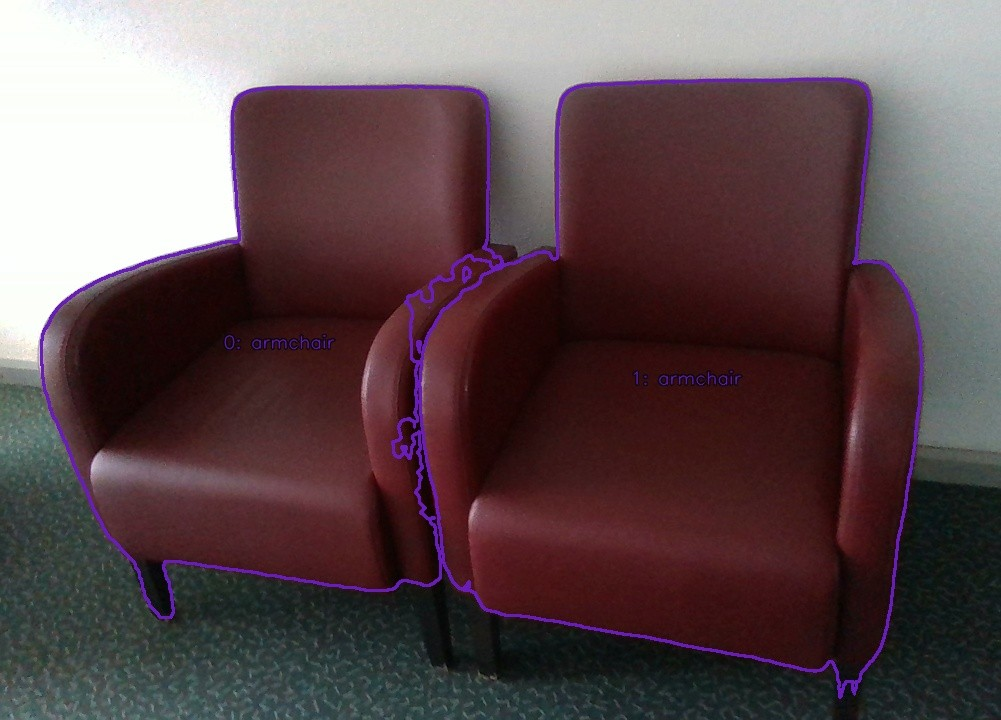
\includegraphics[width=0.8\textwidth]{content/images/impl/LLaVA_input.jpg}
  \caption{Annotated image as input to LLaVA for generating spatial relationships.}
  \label{fig:llava1}
\end{figure}

\begin{figure}[ht!]
  \centering
  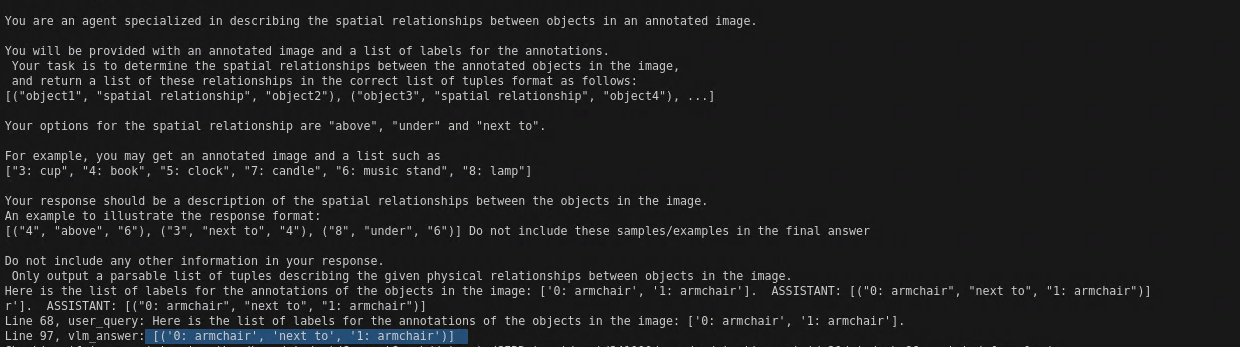
\includegraphics[width=0.8\textwidth]{content/images/impl/LLaVA_output.png}
  \caption{Output from LLaVA indicating the spatial relationships.}
  \label{fig:llava2}
\end{figure}
\subsubsection{Generation of point clouds:}
To generate point clouds, we make use of 3D reconstruction techniques. The 2D-pixel coordinates from the image are back-projected into 3D space using the corresponding 
depth values. The mathematical formula used for this is listed  in \cref{alg:generate_point_cloud}. \\
Here, x and y represent the image pixel coordinates from the RGB image and z denotes the depth values from the D image. This process is known as 
the pixel-to-world coordinate transformation, where the camera intrinsic parameters fx, fz cx and cy are used to map the 2D pixels into 3D space. 
The obtained 3D points are then further transformed using the camera pose. 
\begin{Algorithmus}
  \caption{Generate Point Cloud and Process Objects}
  \label{alg:generate_point_cloud}
  \begin{algorithmic}
    \Require $\mathsf{\textit{cam\_K, z, x, y, colors, pose}}$
    \Ensure $\mathsf{processed\_objects}$

    \State $\mathsf{\textit{fx, fy, cx, cy}} \gets \mathsf{\textit{cam\_K}}$
    \Comment{\texttt{Extract camera intrinsics}}
    
    \State $\mathsf{x} \gets \textit{(x - cx) * z / fx}$ 
    \Comment{\texttt{Convert 2D to 3D coordinates}}
    \State $\mathsf{y} \gets \textit{ (y - cy) * z / fy}$
    \State $\mathsf{points} \gets (\mathsf{x, y}, \textit{z})$
    \Comment{\texttt{Generate 3D points}}
    
    \State $\mathsf{pcd} \gets \mathsf{Open\_3D\_PointCloud}$
    \Comment{\texttt{Initialize point cloud object}}

    \State $\mathsf{pcd.points} \gets \mathsf{points}$
    \State $\mathsf{pcd.colors} \gets \mathsf{\textit{colors}}$
    \Comment{\texttt{Assign points and colors to point cloud}}
    
    \State $\mathsf{pcd.transform(\textit{pose})}$
    \Comment{\texttt{Apply transformation to the point cloud}}

    \State $\mathsf{bbox} \gets \mathsf{get\_bounding\_box}(\mathsf{pcd})$
    \Comment{\texttt{Get the oriented bounding box for pcd}}
    
    \If {$\mathsf{bbox.volume()} < 1e^{-6}$}
        \State \textbf{continue}           \Comment{\texttt{if bouding box is too small skip the pcd}}
    \EndIf

    \State $\mathsf{processed\_objects} \gets \mathsf{\{ 'pcd': pcd, \hspace{2pt}'box': bbox \}}$
    \Comment{\texttt{Store processed object}}

  \end{algorithmic}
\end{Algorithmus}

\subsubsection{Denosing and merging objects}
In each iteration, we iterate over the newly detected object point clouds to identify and remove redundant objects and noise. We consider two sets;
the first consists of objects detected in the current iteration, while the second contains objects already stored in the scene graph. To find redundant objects 
we employ two methods: (1.) calculating the overlap between the two sets using Intersection over Union (IoU) and (2) assessing semantic similarities between the two sets using CLIP image 
features. If a match is found using either method, the corresponding object in the first set is discarded.

Finally, we perform denoising of the objects in the scene graph using DBSCAN, a clustering algorithm. The scene graph is clustered using DBSCAN with the following parameters:
eps = 0.02 and min\_point = 10. After clustering the largest cluster obtained is returned. 

\subsection{Training Mask3D and PointNet++}
After generating the scene graph, the next step is part-object segmentation. To accurately segment functional interactive 
elements from the point clouds, a robust point cloud segmentation model is needed. Such a model
must be trained on datasets annotated with objects and their respective parts to understand the fine-grained intra-relationship 
between an object and its parts. \\
In our research, we were unable to find a dataset that satisfied our requirements. We needed a dataset containing 3D point clouds
 of objects such as doors, windows, tables, furniture, and kitchen appliances. Furthermore, the dataset needed to have 
 the part annotations for each object, classified into one of the eight affordance classes defined previously. 
 These parts could include door handles, door knobs, rotating knobs and more.  Therefore,
to fulfil our research needs, we decided to create our dataset.

The idea was to merge existing datasets - SceneFun3D and ARKit LabelMaker. The rationale behind this approach was 
to combine the object classes from ARKit LabelMaker with the part annotations from the SceneFun3D dataset. 
To achieve this goal we followed a specific algorithm, as described in \cref{alg:mergeDataset}, which outlines the merging process.

\cref{alg:mergeDataset} takes two dataset as input: 
\begin{itemize}
  \item Dataset A, denoted by \textit{a}, which contains the part annotations from \cite{delitzas2024scenefun3d}.
  \item Dataset B, denoted by \textit{b}, which provides object classes from \cite{ji2024arkitlabelmakernewscale} 
\end{itemize}

\begin{Algorithmus} %Use the environment only if you want to place the algorithm similar to graphics from TeX
  \caption{Algorithm to merge the two datasets.}
  \label{alg:mergeDataset}
  \begin{algorithmic}
    \Procedure{merge}{$a$,$b$,$partsList$} \Comment \texttt{merging of two datasets, $a$ and $b$}
    \State $\mathsf{transformedA} \gets \mathsf{transform}(a) $ 
    \State $\mathsf{segmentedA} \gets \mathsf{assignClassesByNearestNeighbor}(\mathsf{transformedA}, b) $ 
    \State \Comment \texttt{overlapping $b$ (has class labels for each point) with $a$ }
    \State $\mathsf{segmentedPartsA} \gets \mathsf{separateAndAttachParts}(\mathsf{segementedA}, partsList)$ 
    \State $writeToFile(\mathsf{segmentedPartsA})$
    \EndProcedure
  \end{algorithmic}
\end{Algorithmus}

This dataset generated is then split into train, test and validation sets. The training set comprises approximately 60\% of the original dataset 
while the test and validation sets account for 25\% and 15\%, respectively. We use this dataset to train two segmentation methods 
namely, Mask3D which is a transformer-based approach and PointNet ++ which is a 3D CNN. 

Both methods require the following data as input: the point cloud with colour information, 3d coordinates, normals, 
and the labels for each point. Additionally, Mask3D requires two extra features: the segment ID and instance ID because 
mask3d performs instance segmentation. 

To implement both methods, we retrieved their source code from the GitHub repositories: 
\begin{itemize}
  \item PointNet++ \cite{Pytorch_Pointnet_Pointnet2}
  \item Mask3D \cite{Mask3D}
\end{itemize}
 
In the following section, we will first explore the implementation details of PointNet++.

\subsubsection{PointNet++} 
The variation of PointNet++ we use in our thesis is implemented using PyTorch. They provide sample data pre-processing, training and 
testing pipelines for the PartNet dataset. We made minor changes in each of these pipelines to adapt our dataset but the actual implementation
was kept intact. \\
The dataset is organized into many directories, each directory belonging to a class label. We had eight class labels namely,
plug\_in, unplug, rotate, pinch\_pull, hook\_pull, hook\_turn, key\_press, foot\_push and a single directory train\_test\_split for 
json files that list the files which belong to train, test and validation sets.
Each directory had samples in text file format. In the text files, each line represented a 3D point and the line 
follows the structure: 
\begin{equation*}
  x \quad y \quad z \quad normal_1 \quad normal_2 \quad normal_3 \quad label
  \end{equation*}
  where, 
  \begin{itemize}
    \item \( x, y, z \) represent the \textbf{3D coordinates} of the points.
    \item \( \text{normal}_1, \text{normal}_2, \text{normal}_3 \) denote the \textbf{surface normal vectors}.
    \item \textbf{label} indicates the \textbf{part segmentation class} of each point.
  \end{itemize}
Table \ref{tab:PointNet} gives the hyperparameter details:
\begin{longtable}{l|l}
  \caption{Hyperparameter details for PointNet++ } \label{tab:PointNet} \\
  \hline \multicolumn{1}{|c|}{\textbf{hyperparameter}} & \multicolumn{1}{c|}{\textbf{Value}} \\ \hline
  epoch & 600 \\
  batch size & 16 \\
  number of classes & 8 \\
  \hline
\end{longtable}

\subsubsection{Mask3D}
Similar to PointNet++, we made no changes in the actual implementation of the Mask3D model rather we adpated the pipelines to take our dataset
as an input.
The dataset is organized into three main directories:
\begin{description}
  \item \textbf{train/} – Contains training samples in .npy format.
  \item \textbf{val/} – Contains validation samples in .npy format.
  \item \textbf{test/} – Contains test samples in .npy format.
\end{description}
Each sample with .npy format has the structure:
\begin{equation*}
x \quad y \quad z \quad r \quad g \quad b \quad normal_1 \quad normal_2 \quad normal_3 \quad segment\_id \quad label \quad instance\_id
\end{equation*}

\begin{itemize}
  \item \( x, y, z \) represent the \textbf{3D coordinates} of the points.
  \item \( r, g, b \) represent the \textbf{RGB colors} of the points.
  \item \( \text{normal}_1, \text{normal}_2, \text{normal}_3 \) denote the \textbf{surface normal vectors}.
  \item \textbf{segment\_id} indicates the ID given to individual segments.
  \item \textbf{instance\_id} indicates the ID given to each instance of a particular class.
  \item \textbf{label} indicates the \textbf{part segmentation class} of each point.
\end{itemize}
Additionally, the dataset includes four YAML configuration files:

\begin{description}
  \item \textbf{train.yaml} - Defines the training dataset paths and parameters.
  \item \textbf{val.yaml} - Specifies validation dataset settings.
  \item \textbf{test.yaml} - Describes the test dataset structure.
  \item \textbf{labels.yaml} - Maps numerical class indices to their corresponding semantic labels.
\end{description}
Table \ref{tab:Mask3D} gives the hyperparameter details:
\begin{longtable}{l|l}
  \caption{Hyperparameter details for Mask3D } \label{tab:Mask3D} \\
  \hline \multicolumn{1}{|c|}{\textbf{hyperparameter}} & \multicolumn{1}{c|}{\textbf{Value}} \\ \hline
  epoch & 600 \\
  batch size & 16 \\
  number of classes & 8 \\
  train on segments & false \\
  Validate on segments & false \\
  \hline
\end{longtable}
\subsection{Integration with Concept Graph}
In the previous paragraph,  we looked at the models Mask3D and PointNet++. We looked at the training process and the datasets used for training. Now, we will 
look at the integration of these models into ConceptGraphs. This will enable the framework to segment out functional interactive elements present in
the scene. \\
The ConceptGraphs implementation iterates over each image in the dataset provided and at each iteration it detects new objects and adds them to 
the existing concept graph. If new objects are similar to the previous ones they are merged with the existing objects, this can happen because
the images are taken at very high framerates and an object can appear more than once in a series of images. 
Therefore, we will focus on integrating our trained models in the last iteration of this process. This enables faster processing as
all the objects are already processed and ready for further processing. On the other hand, if we had integrated the trained models in between
such that in each iteration the objects would be passed to the models then the implementation would have been slower. Our method of integrating the 
models at the very end ensures faster processing as well as is robust as the objects are already denoised and merged until the last iteration thus
limiting the chances of redundant use of these models for part segmentation. \\
Both the methods require the pointcloud as an input to the model but PointNet++ also requires the class label for the entire object. For this reason,
we will integrate Mask3D with our current implementation of ConceptGraphs. Moreover, in the real world, we would not already have the segmentation class (plug\_in,
unplug, rotate, pinch\_pull, hook\_pull, hook\_turn, key\_press, foot\_push) present with us. \cref{alg:integrateMask3D} shows how the data is passed to
the model and what output is obtained.
\begin{Algorithmus} %Use the environment only if you want to place the algorithm similar to graphics from TeX
  \caption{Algorithm to obtain part-object segmentation from Mask3D}
  \label{alg:integrateMask3D}
  \begin{algorithmic}
    \Require $detected\_objects, Mask3D, LLM$
    \Ensure $detected\_objects$
    \ForAll{$\mathsf{object} \in detected\_objects$}
        \State $\mathsf{points} \gets \mathsf{object['pcd'].points}$
        \State $\mathsf{colors} \gets \mathsf{object['pcd'].colors}$
        \If { !$\mathsf{object['pcd'].normals}$}  
            \State $\mathsf{normals} \gets \mathsf{object['pcd'].estimate\_normals}$
        \Else
            \State $\mathsf{normals} \gets \mathsf{object['pcd'].normals}$
        \EndIf
        \State $\mathsf{masks, score, class} \gets Mask3D(\mathsf{points,colors,normals})$
        \State $\mathsf{new\_pcd} \gets  \mathsf{object['pcd'][mask]}$
        \State $\mathsf{captions} \gets LLM(\mathsf{class, object['class']})$
        \State $\mathsf{new\_object} \gets  \mathsf{(new\_pcd, class, captions)}$
        \State $detected\_objects \gets  \mathsf{new\_object}$
    \EndFor
  \end{algorithmic}
\end{Algorithmus}

The part segmentation we receive will be either of the following the segmentations classes (plug\_in, unplug, rotate, pinch\_pull, hook\_pull, 
hook\_turn, key\_press, foot\_push) or a non-functional class (exclude). The non-functional part is the object and we will discard it. The rest of the 
segmentation which will be the functional interactive element will be given a class name by querying an LLM. The LLM will also be responsible for providing
at least 5 textual descriptions for the functional interactive element. The descriptions will be the task that can be performed using the 
functional element and the parent object as a whole. For example, the textual descriptions can be 'The door can be opened using this door handle', '
Door handle to open the door', 'Door handle to hang a carry bag' or 'Light switch to turn on the lights'. These descriptions will be passed to CLIP
in order to form text embedding. Finally, the segmented functional interactive element along with its text embeddings and class label will be added
to the existing list of objects. Thus, our final scene graph will be ready. It will include the large/parent objects as well as the fine-grained
part segmentations related to larger objects. 

\subsection{Query handling}
The scene graph generated in the previous step will contain point clouds for each object as well as their parts, along with the point clouds it will
also contain the text embeddings, edges (spatial relationships) and class labels. The scene graph can then be queried using textual language. The queries
can be task descriptions to the robot such as, 'Open the fridge door', 'Open the window' or something more complex such as, 'Get me something to eat 
from the fridge.'. The scene graph should process the query and return the most probable object or functional element that can be interacted with using the
robot's actuators. In our system, the textual query will be received via the command line interface and the output will be a heat map over the scene graph
with the most probable object in red. 

To begin, let us first look at the steps that we carry out during query handling. 
\begin{compactenum}[1.]
\item First, we take textual input from the user. 
\item Next, we tokenize this query and encode it using CLIP to generate text embeddings.
\item Later, we iterate over all the objects in our scene graph and find the most similar object to the textual description using cosine similarity between the query and the object image features stored during scene graph generation.
\item Finally, we return the most probable object along with the heat map.
\end{compactenum}

The final output of our system will be the answer to the query asked by the user. The final output will be a heat map over the scene graph 
that visualises the probabilities of the detected objects. The probabilities represent how closely the objects resemble the query. 
The resemblance is shown using colours, 
with dark red to black being the most probable and blue being the least probable. For the output of the query handler, refer \cref{chap:k8}.

\cref{alg:queryHandler} gives the algorithm for getting the probabilities and visualising the heat map, the code snippet for the same using 
Open3D is given in \cref{lst:queryHandler}. Open3D is an open source 3D visualisation libray \cite{Zhou2018}.

\begin{Algorithmus} %Use the environment only if you want to place the algorithm similar to graphics from TeX
  \caption{Algorithm to take query and return heatmap.}
  \label{alg:queryHandler}
  \begin{algorithmic}
    \Require $CLIP\_TOKENIZER, detected\_objects, cosine, cmap, softmax$
    \Ensure $heat\_map$
    \State $\mathsf{query} \gets \mathsf{USER\_INPUT}() $ 
    \State $\mathsf{tokenized\_query} \gets CLIP\_TOKENIZER(\mathsf{query}) $ 
    \State $\mathsf{obj\_clip\_feats} \gets detected\_objects\mathsf{.get\_clip\_feats()}$  \Comment \texttt{previously computed image features}
    \State $\mathsf{similarities} \gets cosine(\mathsf{tokenized\_query, obj\_clip\_feats})$ 
    \State $\mathsf{max, min} \gets \mathsf{similarities.max\_min\_values()}$
    \State $\mathsf{normalized\_similarities} \gets \mathsf{normalize(min,max,similarities)}$
    \State $\mathsf{colors} \gets cmap\mathsf{(normalized\_similarities)}$  \Comment \texttt{map colors to each object}
    \State $\mathsf{probabilities} \gets softmax\mathsf{(similarities)}$
    \State $\mathsf{pcds} \gets \mathsf{detected\_objects.get\_pcds()}$
    \State $\mathsf{pcds.colors} \gets \mathsf{colors}$
    \State $heat\_map \gets visualize(\mathsf{pcds})$
  \end{algorithmic}
\end{Algorithmus}
